\section{Data Preparation}
In order to make the data more suitable for the classification task, some preprocessing steps have been applied, including dealing with outliers, checking for possible missing values, column filtering and normalizing the dataset.
%\bigskip
%\subsection{Outlier Detection, Missing Values, Column Filter, Normalizer}
\subsection{Preprocessing and Transformation}
After reading our dataset, we handled numeric \textit{outliers} by using the suited KNIME node, which identifies outliers using the \textit{Interquartile Range (IQR)}. 

After dealing with the outliers, a \textit{missing value} node is used to manage this issue, replacing missing integers and doubles with a median value and dropping rows with missing string values in a column. Even though no missing values were observed in the dataset, this handling is still performed to enable an eventual scalability.

Afterwards, the important features that were determined by Feature Importance process were retained to reduce noise and computations. The \texttt{spec-obj-ID} feature is also maintained: even though it seems to have less importance, it is actually a critical element for differentiating each class, as described in the Section~\ref{sec:ds_desc}. 

Then, we have applied Z-score normalization on the selected columns to scale our data such that the values are normally distributed. This ensured that no single feature affected the model disproportionally.
%Since our dataset is an unbalanced data set, meaning that some classes have objectively more values than the others, undersampling has been applied to the majority class in order to make the values more balanced. Equal Size Sampling node is used for this purpose. Normalizer node is used to transform the values into a consistent state. This ensured that no single feature affected the model disproportionally. SMOTE is also used throughout the design in order to produce synthetic values in order to further balance the dataset.
\subsection{Exploratory Data Analysis}
Exploratory data analysis methodologies are applied in order to visualize the data distributions and correlations, and improve understanding beforehand. 

We mainly produced a linear correlation matrix (as visible in Fig.~\ref{fig:corrmatrix}) between features, and it emerged that the features with the highest correlation values with \texttt{class} are \texttt{u}, \texttt{g} and \texttt{redshift}.
\vspace{-1.5cm}
\begin{figure}[H]
    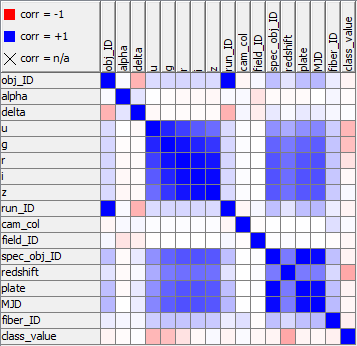
\includegraphics[width=0.9\columnwidth]{images/Correlation Matrix.png}
    \centering
    \caption{Feature correlation matrix.}
    \label{fig:corrmatrix}
\end{figure}
\vspace{-3cm}
The exploration of the relationship of \texttt{u} and \texttt{g} with other features displayed difficulties for determining the class of the observations. Despite this, we decided to further explore \texttt{redshift} against other features, and this led to the conclusion that \texttt{redshift} is the most significant feature to classify our records.
%\vspace{-0.3cm}
\subsection{Feature Importance}
Feature importance has been applied to detect the most important features and use them to reduce computations and noise, without losing relevant information. This has been implemented with Tree Ensemble, which learns an ensemble of decision trees, such as Random Forest variants. This method gave us an importance score for each feature, allowing us to understand their relative significance in the classification task.   
\begin{figure}[H]
    \centering
    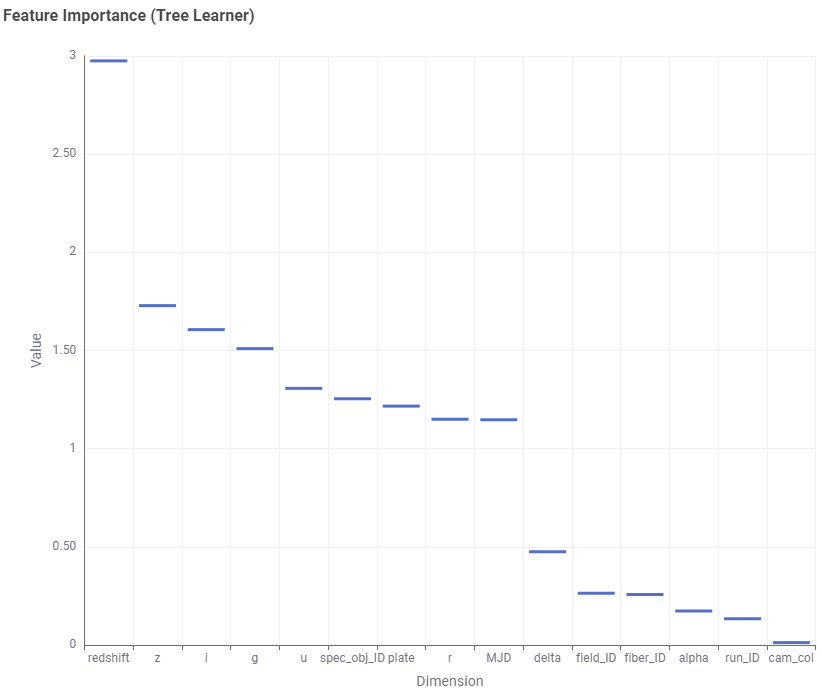
\includegraphics[width=1\columnwidth]{images/Feature Importance.png}
    \caption{Feature Importance based on Tree Learner.}
    \label{fig:fig2}
\end{figure}
We used every feature with a score value greater than 1, except for \texttt{MJD} and \texttt{plate}.\\We excluded these two because it turned out that they do not affect performance at all.